\documentclass[article,nontitlepage,]{dennou777}

\ltjsetparameter{jacharrange={-2}}%ギリシア文字、キリル文字を AL Char に。
\usepackage[no-math,match,deluxe,fontspec,jfm_yoko=jlreq,jfm_tate=jlreqv]{luatexja-preset}

\usepackage[T1]{fontenc}
\usepackage{yhmath,amsmath,mathtools,amssymb,mathrsfs,rsfso,mleftright}
\usepackage[math]{kurier}
\usepackage[euler-digits]{eulervm}
\usepackage[scaled]{beramono}
%\usepackage{classico,newpxtext}
\DeclareMathAlphabet{\mathtt}{T1}{fvm}{m}{n}
\DeclareMathAlphabet{\mathsf}{T1}{uop}{m}{n}

\usepackage[unicode,colorlinks]{hyperref}
\hypersetup{linkcolor=,urlcolor=teal}

\usepackage{pxrubrica}

\usepackage{autobreak}

\usepackage{tcolorbox}

\setmainfont{Exo 2}
\setsansfont{Exo 2}
\setmainjfont{FOT-MatissePro-DB}[
	AltFont={
		{
			Range={
				"4E00-"9FFF, % CJK 統合漢字
				"3400-"4DFF, % CJK 統合漢字拡張 A
				"20000-"2EBE0, % CJK 統合漢字拡張 B-F
				"2460-"24FF, % 囲み英数字
				"3200-"32FF, % 囲み CJK 文字・月
				"1F100-"1F2FF % 囲み英数字補助、漢字補助
			},
			Font=FOT-RodinNTLGPro-DB,
		},
	},
	BoldFeatures={
		Font=FOT-MatissePro-EB,
		AltFont={
			 {
				Range={
					"4E00-"9FFF, % CJK 統合漢字
					"3400-"4DFF, % CJK 統合漢字拡張 A
					"20000-"2EBE0, % CJK 統合漢字拡張 B-F
					"2460-"24FF, % 囲み英数字
					"3200-"32FF, % 囲み CJK 文字・月
					"1F100-"1F2FF % 囲み英数字補助、漢字補助
				},
				Font=FOT-RodinNTLGPro-EB,
			},
		},
	},
	YokoFeatures={JFM=jlreq},   % jlreqのJFMを維持する
	TateFeatures={JFM=jlreqv},  % https://qiita.com/zr_tex8r/items/91ae1dcc9c3afce7fa8c
]
\setsansjfont{FOT-RodinNTLGPro-DB}[
	AltFont={
		{
			Range={
				"4E00-"9FFF, % CJK 統合漢字
				"3400-"4DFF, % CJK 統合漢字拡張 A
				"20000-"2EBE0, % CJK 統合漢字拡張 B-F
				"2460-"24FF, % 囲み英数字
				"3200-"32FF, % 囲み CJK 文字・月
				"1F100-"1F2FF % 囲み英数字補助、漢字補助
			},
			Font=FOT-RodinNTLGPro-DB,
		},
	},
	BoldFeatures={
		Font=FOT-MatissePro-EB,
		AltFont={
			 {
				Range={
					"4E00-"9FFF, % CJK 統合漢字
					"3400-"4DFF, % CJK 統合漢字拡張 A
					"20000-"2EBE0, % CJK 統合漢字拡張 B-F
					"2460-"24FF, % 囲み英数字
					"3200-"32FF, % 囲み CJK 文字・月
					"1F100-"1F2FF % 囲み英数字補助、漢字補助
				},
				Font=FOT-RodinNTLGPro-EB,
			},
		},
	},
	YokoFeatures={JFM=jlreq},   % jlreqのJFMを維持する
	TateFeatures={JFM=jlreqv},  % https://qiita.com/zr_tex8r/items/91ae1dcc9c3afce7fa8c
]\setmonofont[
	Ligatures=TeX,
	Scale=0.89,
]{DejaVu Sans Mono}
\setmonojfont[
	Ligatures=TeX,
	Scale=0.89,
]{NotoSansMonoCJKjp-Regular}

\allowdisplaybreaks[4]
\ltjenableadjust[lineend=extended,priority=true,profile=true,linestep=true]

%%%%%%%%%%%%自作マクロ

%%matrix
\newcommand{\Mtx}[1]{\begin{matrix} #1 \end{matrix}}
\newcommand{\pMtx}[1]{\begin{pmatrix} #1 \end{pmatrix}}
\newcommand{\bMtx}[1]{\begin{bmatrix} #1 \end{bmatrix}}
\newcommand{\BMtx}[1]{\begin{Bmatrix} #1 \end{Bmatrix}}
\newcommand{\vMtx}[1]{\begin{vmatrix} #1 \end{vmatrix}}
\newcommand{\VMtx}[1]{\begin{Vmatrix} #1 \end{Vmatrix}}

\newcommand{\hmvec}{\mathbold}
\newcommand{\eqdef}{\stackrel{\mathrm{def}}{=}}
\newcommand{\centeralign}[1]{\rule{0pt}{0pt}\hfill#1\hfill\rule{0pt}{0pt}}
\newcommand{\Unit}[1]{\,\mathrm{#1}}

\Dtitle[大気放射の基礎]{大気放射の基礎\\--Liou著 藤枝・深堀訳 (2014) の講読--}
\Dauthor[人見祥磨]{北海道大学理学部 地球惑星科学科 宇宙惑星グループ\\02160611 人見祥磨}

\begin{document}
\maketitle

\tableofcontents

\section{動機}

\subsection{動機}
\begin{itemize}
	\item 惑星大気の熱輸送について興味があった
	\item 惑星大気について、自転周期や地軸の傾きによって、
		どのように熱輸送が変化するかシミュレーションしたい
	\item そのために、大気の温度分布を知りたい
	\item 放射に関する基本的な事項の知識の確認
	\item 放射に関して、観測なども含めて、基礎事項を解説している Liou の教科書を
		読むことにした
		\begin{itemize}
			\item 大気放射学 {\scriptsize---衛星リモートセンシングと気候問題へのアプローチ---}\\
				K.N.Liou(著) 藤枝 鋼、深堀 正志(翻訳)\\
				共立出版 \textbf{(2014)} 672ページ
		\end{itemize}
\end{itemize}

\section{基本的な放射量}

放射が進行することで、放射は相互作用により増減する。これを記述する
\textbf{放射伝達方程式}を導くことが目的である。

そのために、放射量を表すための物理量の定義について確認する。

\subsection{基本的な放射量}
\begin{description}
	\item[単色の放射強度 $I_\lambda$]\leavevmode\\
		面積 $dA$ を横切り、$dA$ の法線からなす角 $\theta$ の方向にある
		微小立体角 $d\Omega$ から入射する、ある波長区間 $\lambda$ 〜
		$\lambda+d\lambda$ における、微小時間 $dt$ の間の微小放射エネルギー量
		$dE_\lambda$
		\[dE_\lambda=I_\lambda\cos[\theta]\,dA\,d\Omega\,d\lambda\,dt\]
		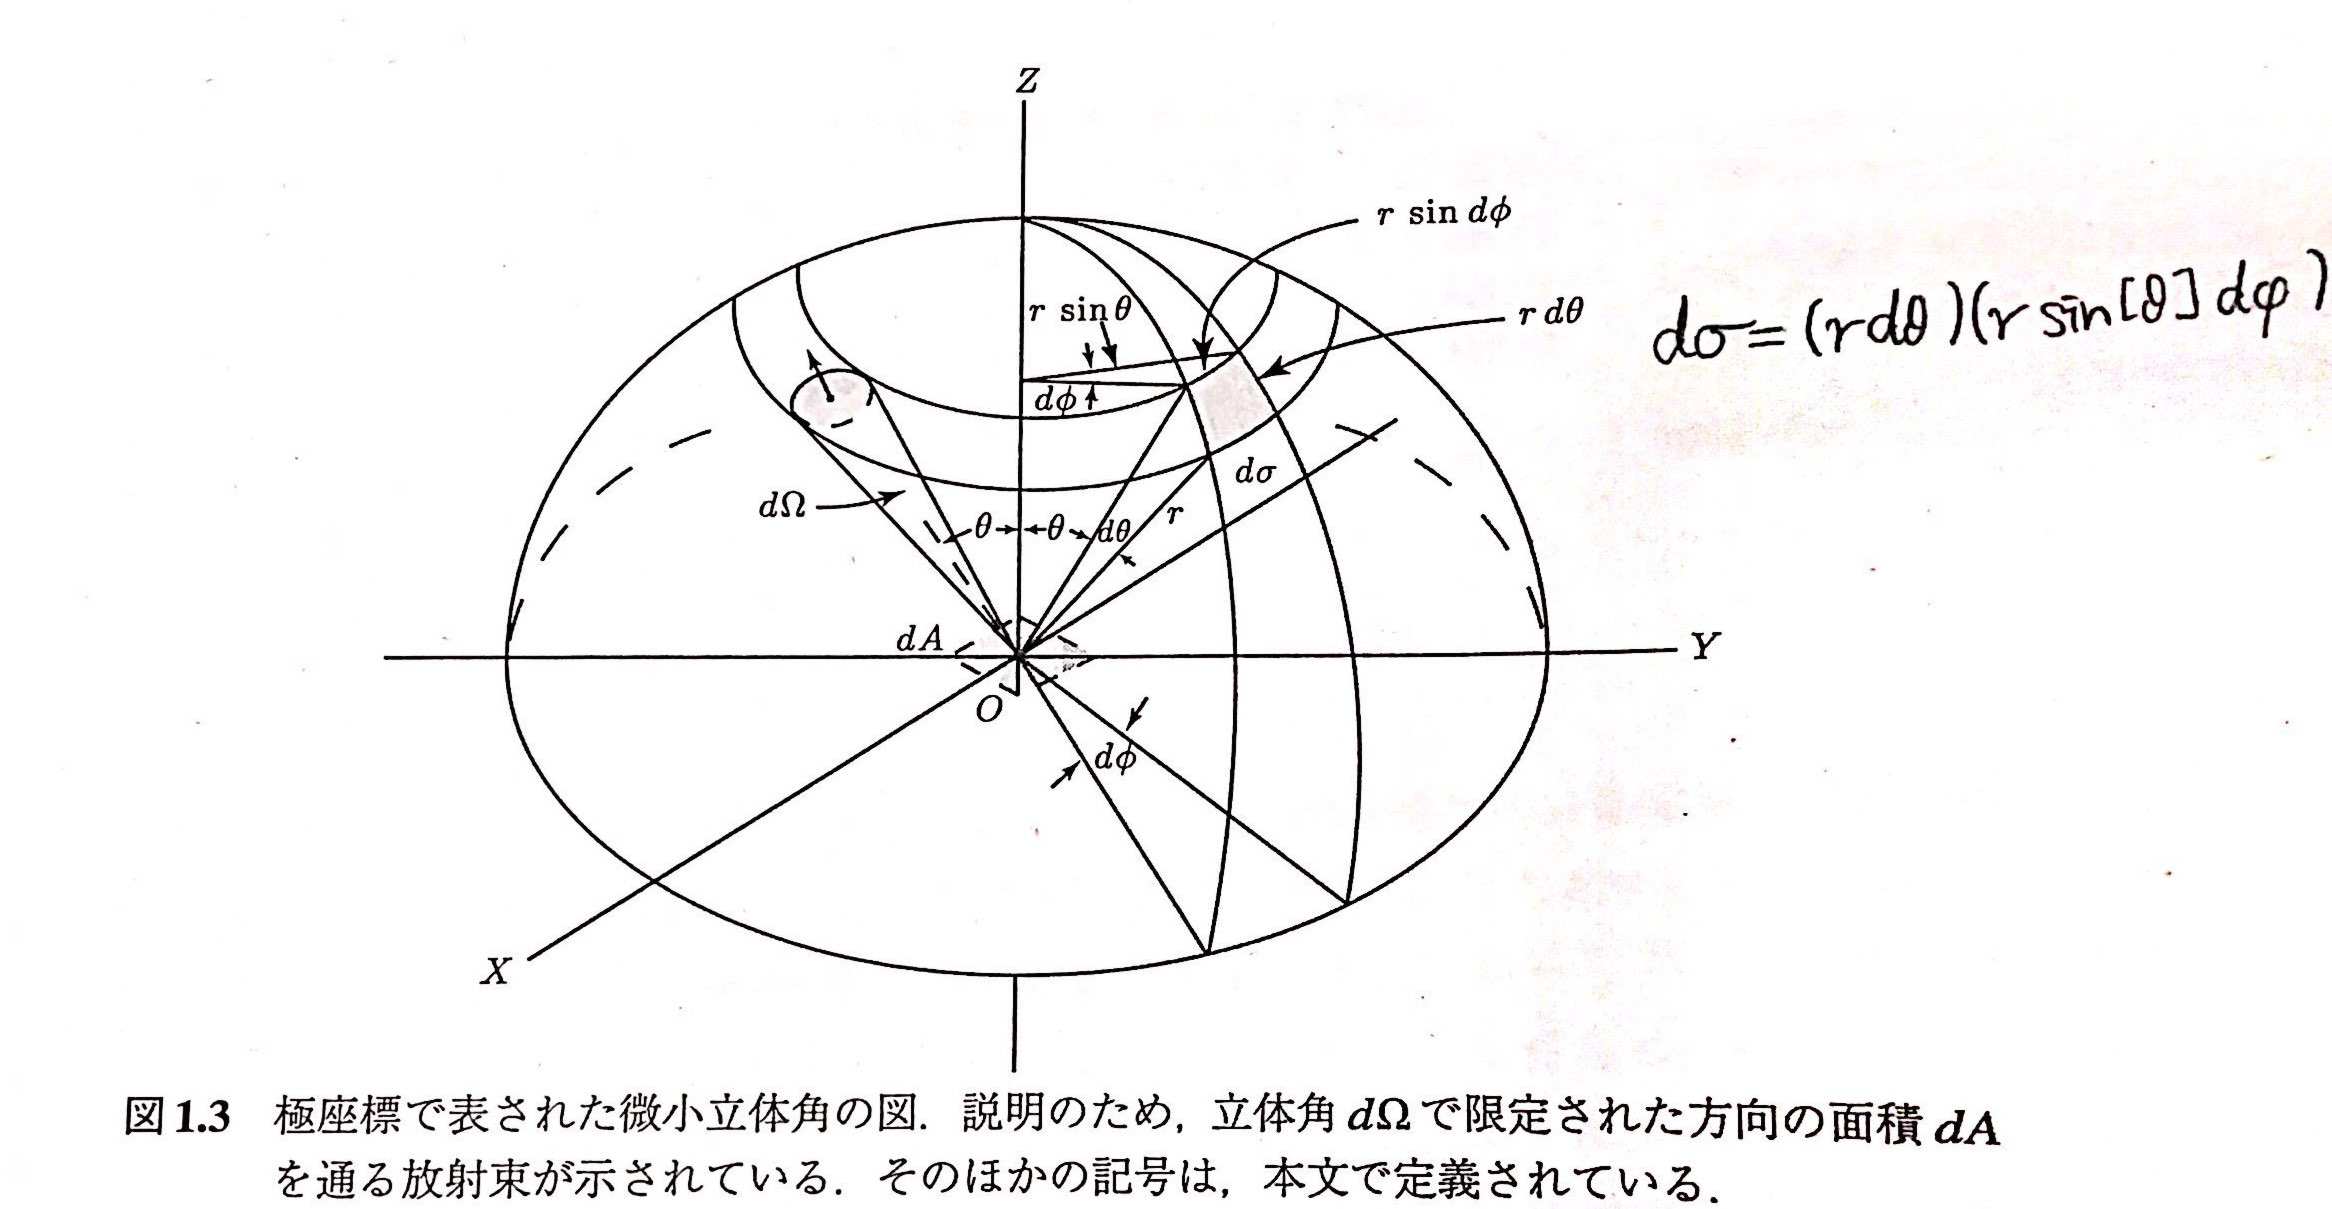
\includegraphics[width=\linewidth]{eq.jpg}
\end{description}

\begin{description}
	\item[単色の放射フラックス密度 $F_\lambda$]\leavevmode\\
		単色の放射輝度を、半球の全立体角にわたって積分したものの、法線成分
		\[F_\lambda=\int_\Omega I_\lambda\cos[\theta]\,d\Omega\]
	\item[全放射フラックス密度 $F$]\leavevmode\\
		単色の放射フラックス密度を、波長全体で積分
		\[F=\int^\infty_0 F_\lambda\,d\lambda\]
	\item[全放射フラックス $f$]\leavevmode\\
		全放射フラックス密度を、面全体で積分
		\[f=\int_AF\,dA\]
\end{description}

\section{散乱と吸収の概念}
放射は、散乱や吸収の過程を経て、強度が変化する。

このことは、放射伝達方程式に記述されるが、実際にどのような現象が
発生しているか確認する。

\subsection{散乱と吸収の概念}
\begin{description}
	\item[散乱] 入射波と衝突した粒子が、入射した電磁波のエネルギーを、あらゆる方向に
		再放射する過程。すべての波長で発生し、粒子の大きさが影響する。
		\begin{description}
			\item[独立散乱] 粒子が少ないとき、個々の粒子が全く同じように散乱する。
			\item[多重散乱] 粒子が多量にあるとき、散乱が繰り返される。\\
				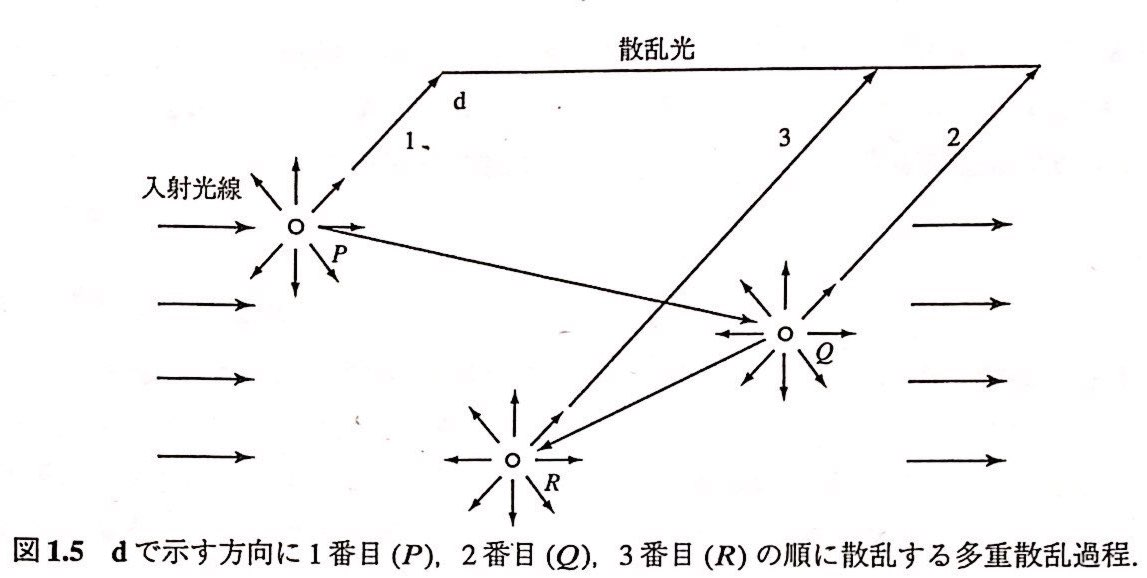
\includegraphics[width=\linewidth]{mscatter.jpg}
		\end{description}
\end{description}

\subsection{散乱の種類}
散乱にはサイズパラメーター $x=2\pi a/\lambda$ ($a$ は粒径)が影響する。

\centeralign{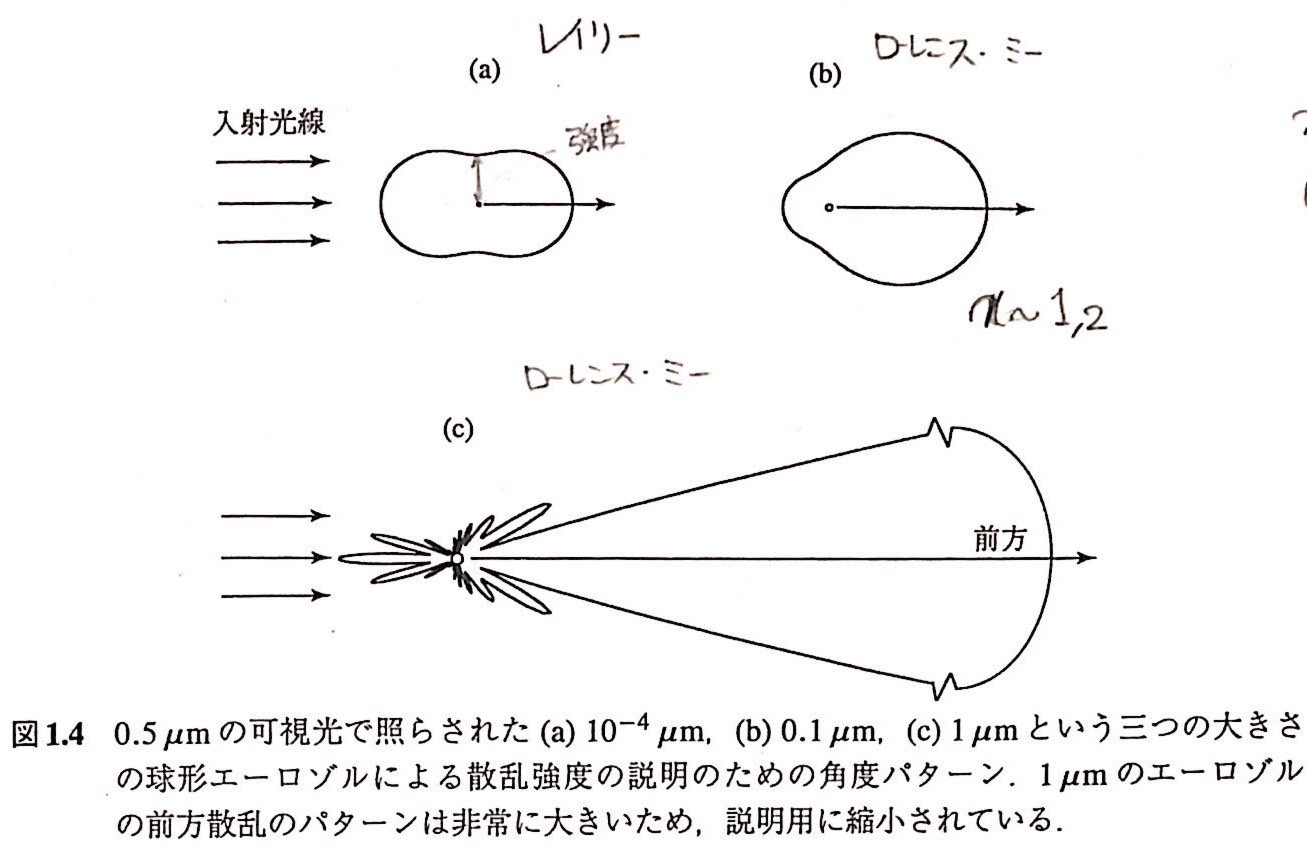
\includegraphics[width=0.8\textwidth]{scatter.jpg}}

\section{黒体放射の法則}

黒体とは吸収のない理想的な物体である。
放射を考える上で、最も基本的な物体として黒体を考える。

黒体の放射を支配する 4 つの法則について述べる。

\subsection{プランクの法則}
振動子が持つエネルギーは $E=nh\tilde{\nu}$ に量子化されると仮定する。

プランク関数: $\displaystyle B_{\tilde{\nu}}[T]=\frac{2h\tilde{\nu}^3}{c^2(\exp[h\tilde{\nu}/k_\mathrm{B}T]-1)}$\\
{\scriptsize ($\tilde{\nu}$: 周波数、$h$: プランク定数、$k_\mathrm{B}$: ボルツマン定数、
$c$: 光速、$T$: 絶対温度)}

射出された単色の放射強度を、周波数と射出する物質の温度に関連付ける

波長$\lambda$に関するプランク関数:
\[B_\lambda[T]=\frac{2hc^2}{\lambda^5(\exp[hc/k_\mathrm{B}\lambda T]-1}=
	\frac{C_1\lambda^{-5}}{\pi(\exp[C_2/\lambda T]-1)}\]
{\scriptsize ($C_1=2\pi hc^2, C_2=hc/k_\mathrm{B}$)}

\subsection{プランクの法則}
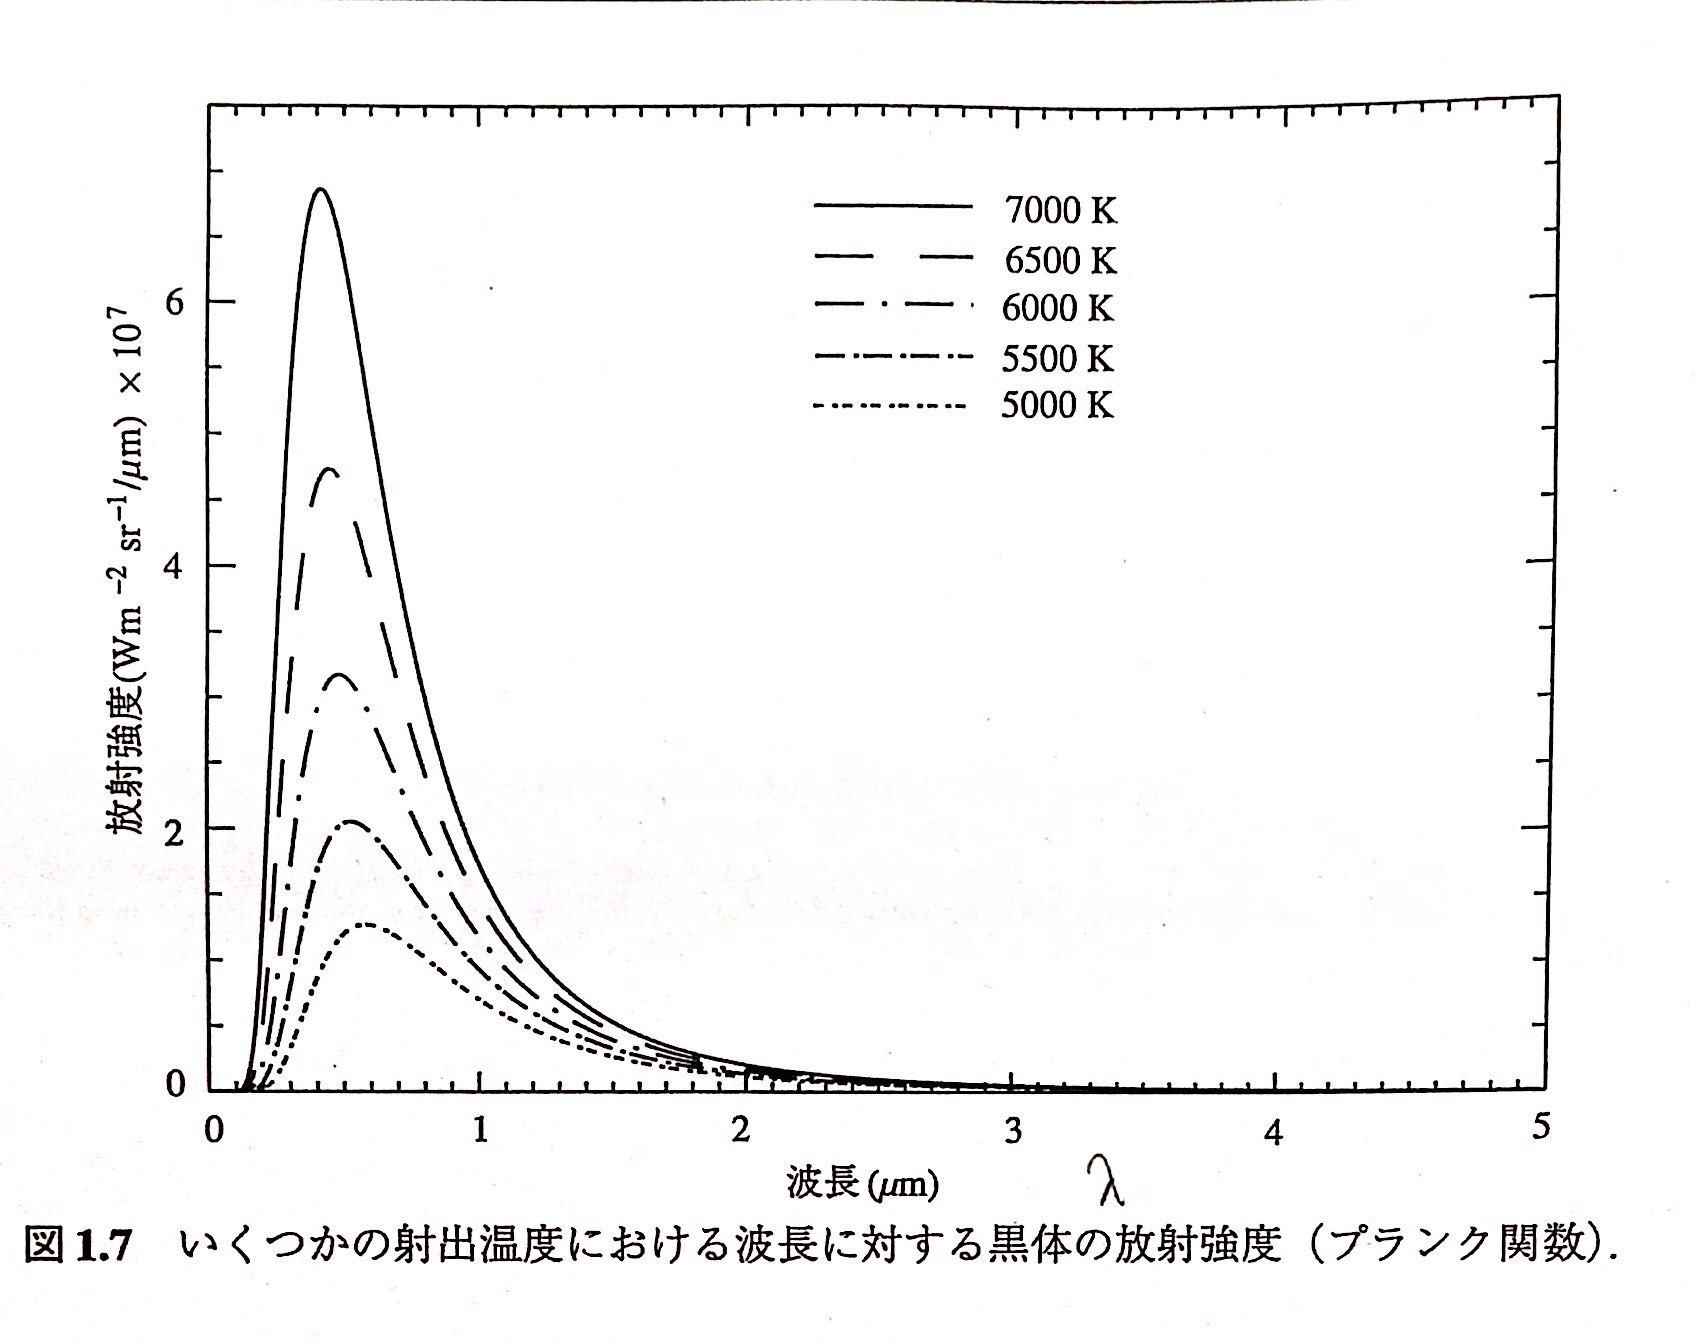
\includegraphics[width=\textwidth]{planck.jpg}

\subsection{ステファン・ボルツマンの法則}
黒体の全放射強度: プランク関数を波長全体で積分

\[B[T]=\int^\infty_0 B_\lambda[T]\,d\lambda=bT^4, \qquad b=\frac{2\pi^4k_\mathrm{B}^4}{15c^2h^3}\]

等方な黒体によって放射される放射フラックス密度: \[F=\pi B[T]=\sigma T^4\]
$\sigma=5.67\times10^{-8}\Unit{J\,m{-2}\,s^{-1}\,k_\mathrm{B}^{-4}}$; ステファン・ボルツマン定数

広い波長域での赤外放射伝達の解析の基礎となる

\subsection{ウィーンの変位則}
黒体放射の最大放射強度の波長が、温度に反比例する

\[\frac{\partial B_\lambda[T]}{\partial\lambda}=0\quad\text{これを解くと}\quad\lambda_m=\frac{a}{T}\]
($a=2.897\times10^{-3}\Unit{m\,K}$; ウィーンの変位定数)

\subsection{キルヒホッフの法則}
以下の条件を満たしているとき、射出と吸収が等しくなる

\begin{itemize}
	\item 一様な温度
	\item 等方性放射
	\item 熱力学的平衡
\end{itemize}

中間圏よりも高度が低い、局所的に限られた空間では、
エネルギー遷移が分子の衝突によって支配される範囲内で、精度良く成り立つと考えて良い

\section{放射伝達の基礎}
ある方向に進む放射が、吸収や散乱などの相互作用で、どのように増減するか
記述するのが、放射伝達方程式である。

放射伝達方程式を導き、特定の状況での放射伝達方程式の解を求める。

\subsection{放射伝達方程式}
放射伝達強度 $I_\lambda^\mathrm{d}$ が、放射の伝搬方向に厚さ $ds$ で密度 $\rho$ の媒質を横切った後に、
$I_\lambda^\mathrm{d}+dI_\lambda^\mathrm{d}$ になるとする
\[dI_\lambda^\mathrm{d}=-k_\lambda\rho i_\lambda\,ds\]
$k_\lambda$ は質量消散断面積と呼ばれる

射出と多重散乱による放射強度の増加が以下で与えられるように、
放射源係数 $j_\lambda$ を定義する
\[dI_\lambda^\mathrm{s}=j_\lambda\rho\,ds\]

\subsection{放射伝達方程式}
ふたつの式を関連付けて、
\[dI_\lambda=dI_\lambda^\mathrm{d}+dI_\lambda^\mathrm{s}=-k_\lambda\rho I_\lambda\,ds+j_\lambda\rho\,ds\]

放射源関数 $J_\lambda\equiv j_\lambda/k_\lambda$ を導入すると、
\[\frac{dI_\lambda}{k_\lambda\rho\,ds}=-I_\lambda+J_\lambda\quad\text{……放射伝達方程式}\]

\subsection{ビーアー・ブーゲー・ランバートの法則}
大気系からの射出の寄与を無視できる
\[\frac{dI_\lambda}{k_\lambda\rho\,ds}=-I_\lambda\]

積分すると
\[I_\lambda[s_1]=I_\lambda[0]\exp[-k_\lambda u],\qquad u=\int^{s_1}_0\rho\,ds\quad\text{(光路長)}\]

一様に消散する媒質を横切る放射強度の低下が、質量消散断面積と
光路長の積の指数関数に従う

\subsection{シュワルツシルトの方程式}
地球と大気から射出される熱赤外放射伝達\\
放射源関数はプランク関数で与えられる

放射伝達方程式: シュワルツシルトの式
\[\frac{dI_\lambda}{k_\lambda\rho\,ds}=-I_\lambda+B_\lambda[T]\]

シュワルツシルトの式の解:
\[I_\lambda[s_1]=I_\lambda[0]\exp\bigl[-\tau_\lambda[s_1,0]\bigr]+
	\int^{s_1}_{0}B_\lambda\bigl[T[s]\bigr]\exp\bigl[-\tau_\lambda[s_1,s]\bigr]k_\lambda\rho\,ds\]
\[\tau_\lambda[s_1,s]=\int^{s_1}_s k_\lambda\rho\,ds\qquad\text{($s$ と $s_1$ の間の光学的厚さ)}\]

\section{まとめ}

\subsection{まとめ・今後の展望}
\begin{itemize}
	\item 基礎方程式の概念がわかった
	\item 特定の状況(大気系からの射出を無視できる場合や、シュワルツシルトの方程式)
		での、放射伝達方程式の解法を学んだ
	\item 放射伝達方程式から計算できるもの
		\begin{itemize}
			\item 放射伝達方程式から吸収の鉛直分布を求めることができる
			\item その結果、気温の鉛直分布がわかるようになる
		\end{itemize}
	\item 実際に応用する方法がわかっていないので、第 8 章を読み進めているところ
\end{itemize}

\section{スペクトル線の広がり}
単色の放射は、相互作用により非単色となり、有限の幅を持つスペクトル線となる

\subsection{スペクトル線の広がり}
単色の射出は現実には観測されない

原子や分子への外部からの影響と、射出の際のエネルギー損失のため、
エネルギー遷移する間にエネルギー準位が僅かに変化する

その結果、非単色の放射となり、有限の幅を持つスペクトル線が観測される

\subsection{ローレンツ線形}
\begin{description}
	\item[ローレンツ線形] 衝突によって広げられたスペクトル線の線形
\end{description}

\[k_\nu=\frac{S}{\pi}\frac{\alpha}{(\nu-\nu_0)^2+\alpha^2}=Sf[\nu-\nu_0]\]
\centeralign{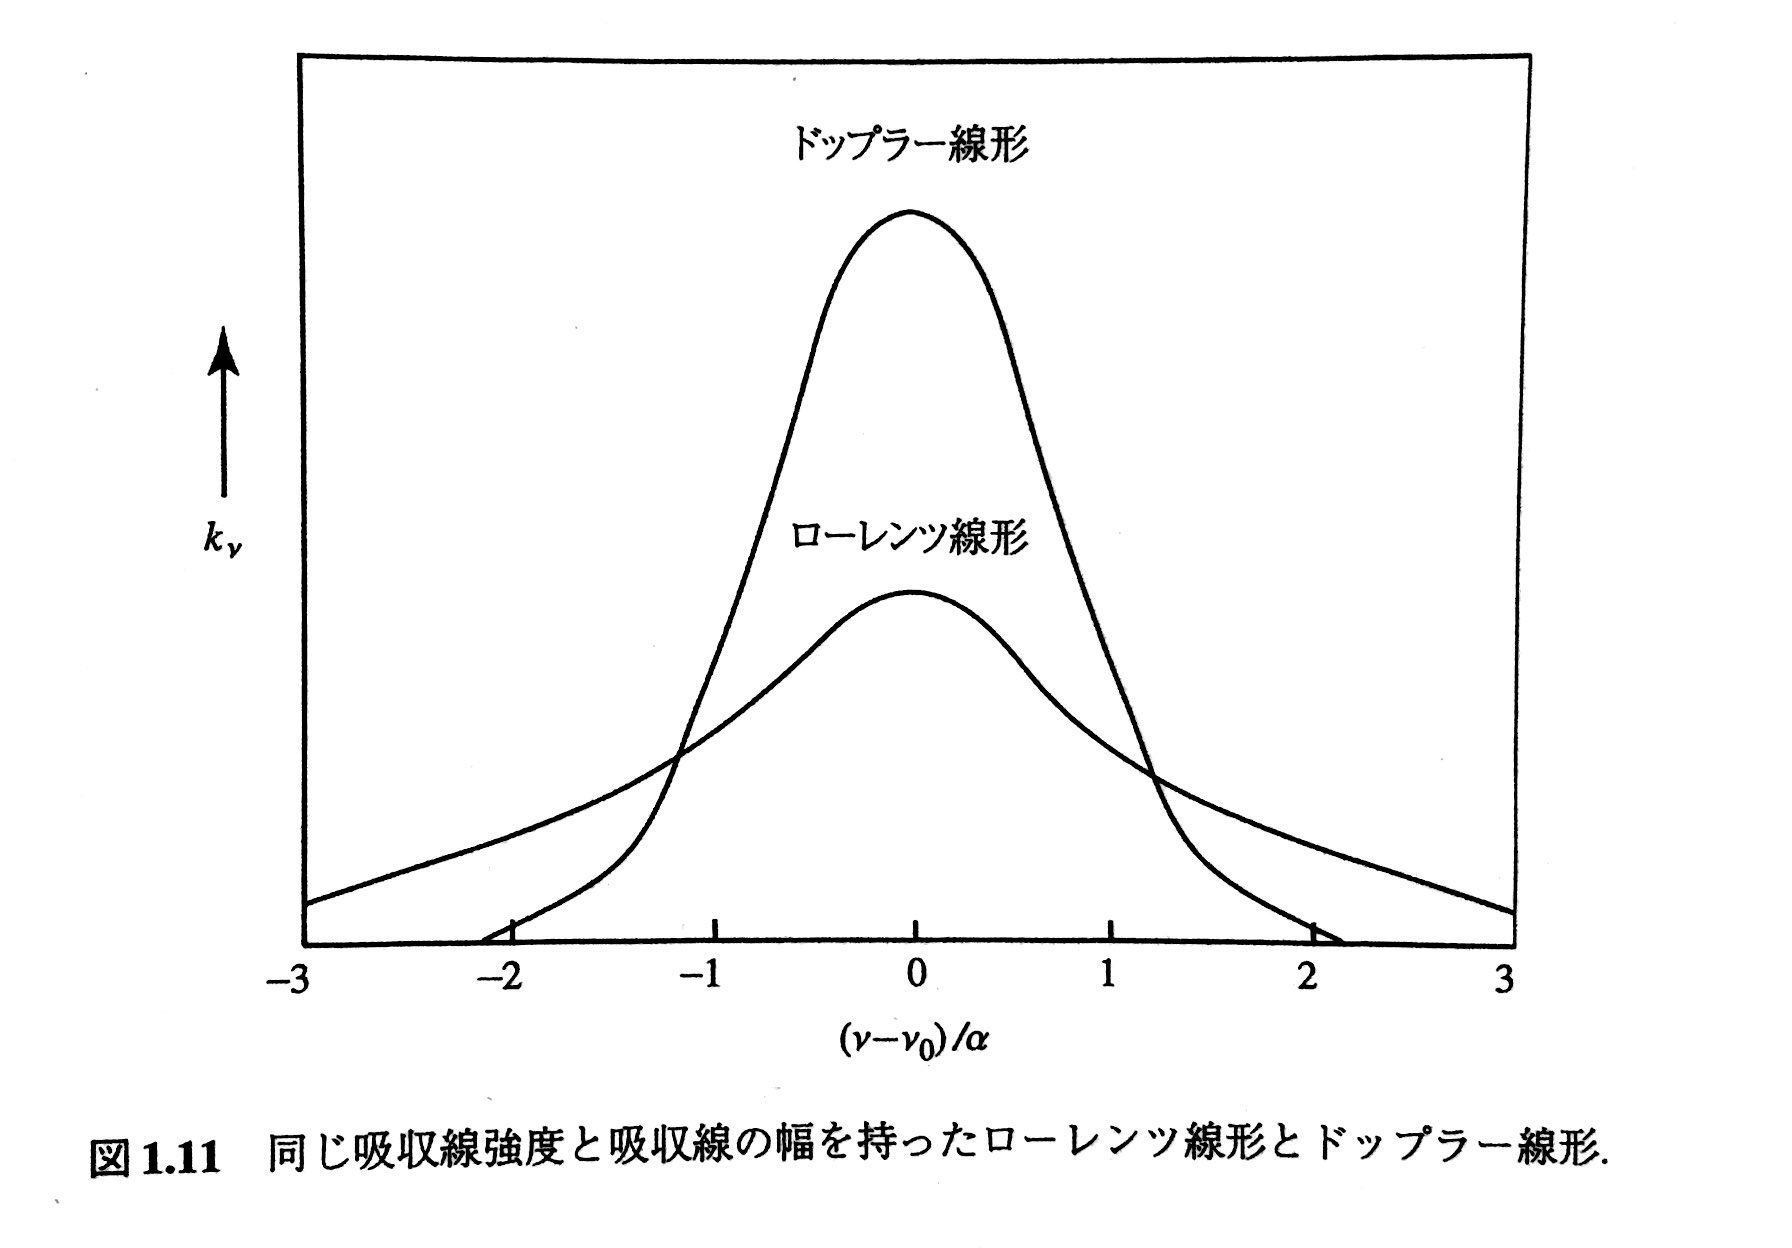
\includegraphics[width=\textwidth]{lorentz.jpg}}

$k_\nu$: 吸収係数 ;\quad
$\nu_0$: 理想的な単色の吸収線の波数;\\
$\alpha$: 吸収線の半値半幅(圧力と温度の関数);\\
$f$: 形状因子 (shape factor);\quad
$\displaystyle S=\int^\infty_{-\infty}k_\nu\,d\nu$: 線強度

\section{大気の熱赤外放射伝達}
放射伝達方程式から、大気の放射フラックス密度を形式的に得る

\subsection{大気の熱赤外放射伝達}
\subsubsection{放射に関してのバランス方程式}
ステファン・ボルツマンの法則から
\[S\cdot\pi{a_e}^2(1-\bar r)=\sigma{T_e}^4\cdot4\pi{a_e}^2\]
アルベド: $\bar r$;\quad 地球半径: $a_e$;\quad\\
太陽定数: $S=1366\Unit{W\,m^{-2}}$;\quad 地球大気系の平衡温度: $T_e$

バランス方程式より、
\[T_e=\sqrt[4]{S\frac{1-\bar r}{4\sigma}}\sim255\Unit{K}\]

\subsection{放射伝達のための一般的な方程式}
放射束の放射強度: $I_\nu$;\quad 吸収係数: $k_\nu$;\\
吸収気体の密度: $\rho_a$;\quad 光路長: $s$;\quad 放射源関数: $J_\nu$
\[-\frac{1}{k_\nu \rho_a}\frac{dI_\nu}{ds}=I_\nu-J_\nu\]

\begin{description}
	\item[放射強度] 時間に依存しないと仮定
	\item[平行平面大気] 放射強度と大気パラメーターは鉛直方向にのみ変化
\end{description}

\subsection{$\tau$ 座標に変換}
放射強度は天頂角と鉛直位置のみの関数\\
$B_\nu[z]=B_\nu[T[z]]$ はプランク放射強度
\[-\mu\frac{dI_\nu[z,\mu]}{k_\nu\rho_a\,dz}=I_\nu[z,\mu]-B_\nu[z]\]

光学的深さ $\tau$ を導入($p=\rho_a/\rho$ は気体の混合比)
\[\tau=\int^{\mathrm{TOA}}_{z} k_\nu[z]\rho_a[z]\,dz=\int^p_0 k_\nu[p]q[p]\frac{dp}{g}\]
\[d\tau=-k_\nu[z]\rho_a[z]\,dz=k_\nu[p]q[p]dp/g\]

放射伝達方程式を $\tau$ 座標に変換
\[\mu\frac{dI_\nu[\tau,\mu]}{d\tau}=I_\nu[\tau,\mu]-B_\nu[\tau]\]

\subsection{境界条件}
境界条件: 地球表面からの射出と大気上端 (TOA) からの射出が等方性となる

全光学的厚さ: $\tau_*$

地球表面は赤外で黒体と仮定 $I_\nu[\tau_*,\mu]=B_\nu[\tau_*]$

大気上端では $I_\nu[0,-\mu]=B[\mathrm{TOA}]\simeq0$ と仮定

\subsection{放射強度の型式解}
単色の透過率 $T_\nu[\tau/\mu]=e^{-\tau/\mu}$ を定義

放射強度の型式解は
\begin{align*}
	I^\uparrow_\nu[\tau,\mu]
		&=B_\nu[\tau_*]T_\nu\left[\frac{\tau_\nu-\tau}{\mu}\right]
		-\int^{\tau_*}_\tau B_\nu[\tau']\frac{d}{d\tau'}T_\nu\left[\frac{\tau'-\tau}{\mu}\right]d\tau'\\
	I^\downarrow_\nu[\tau,-\mu]
		&=\int^\tau_0 B_\nu[\tau']\frac{d}{d\tau'}T_\nu\left[\frac{\tau-\tau'}{\mu}\right]d\tau'
\end{align*}

大気の加熱率の計算に必要な放射フラックス密度は、上半球と下半球の放射強度の和
\[F^{\uparrow\downarrow}_\nu[\tau]=2\pi\int^1_0 I^{\uparrow\downarrow}_\nu[\tau,\pm\mu]\mu\,d\mu\]

\subsection{大気の放射フラックス密度}
角度方向の積分を考慮するため、拡散透過率 $T^f_\nu$ を導入
\[T^f_\nu[\tau]=2\int^1_0 T_\nu\left[\frac{\tau}{\mu}\right]\mu\,d\mu\]

\begin{align*}
	F^\uparrow_\nu[\tau]
		&=\pi B_\nu[\tau_*]T^f_\nu[\tau_*-\tau]
		-\int^{\tau_*}_\tau \pi B_\nu[\tau']\frac{d}{d\tau'}T^f_\nu[\tau'-\tau]d\tau'\\
	F^\downarrow_\nu[\tau]
		&=\int^\tau_0 \pi B_\nu[\tau']\frac{d}{d\tau'}T^f_\nu[\tau-\tau']d\tau'
\end{align*}

放射フラックスの波数積分は、$\tau$ が波数の関数なので、
\[F^{\uparrow\downarrow}[z]=\int^\infty_0 F^{\uparrow\downarrow}_\nu[z]\,d\nu\]
光学的深さに沿った波数積分を必ず含む

\subsection{ラインバイライン積分}
ある与えられた波数と分子種には、さまざまな吸収線の吸収係数が透過率へ寄与する
\[\tau=\sum_j \tau_j=\int_u\sum_j k_{\nu,j}[u]\,du\]

したがって、吸収係数は吸収線強度と吸収線形の式で表すことができる
\[k_\nu[p,T]=\sum_j S_j[T]f_{\nu,j}[p,T]\]

\subsection{分光透過率}
赤外放射伝達の計算をする際は、プランク関数の変動が無視しうるような
小さな波数区間で放射パラメーターを決めることが有効

放射強度と放射フラックスの方程式における基本的な放射パラメーターとして、
平均波数の添字 $\bar\nu$ のついた分光透過率を定義する
\[
	T_{\bar\nu}[u]
	=\int_{\Delta\nu}\exp[-\tau]\frac{d\nu}{\Delta\nu}
	=\int_{\Delta\nu}\exp\left[-\int_u\sum_j k_{\nu,j}[u]\,du\right]\frac{d\nu}{\Delta\nu}
\]

\section{相関 $k$ 分布法}

\subsection{相関 $k$ 分布法}
気体の分光透過率を吸収係数 $k_\nu$ に応じてグループとして扱う

均質な大気では分光透過率は吸収係数 $k$ の順序に依存しない\\
波数積分は $k$ 空間での積分に置き換えることができる

\subsection{相関 $k$ 分布法}
波数区間 $\Delta\nu$ における $k_\nu$ に対する正規化確率密度関数が
$f[k]$ で与えられ、その最大値と最小値がそれぞれ $k_{\mathrm{min}}\to0$、
$k_{\mathrm{max}}\to\infty$ だとすると、分光透過率は
\[T_{\bar\nu}[u]=\int_{\Delta\nu}\exp[-k_\nu u]\frac{d\nu}{\Delta\nu}=\int^\infty_0 \exp[-ku]f[k]\,dk\]

確率密度関数 $f$ は分光透過率のラプラス逆変換であるとわかる
\[f[k]=\mathcal{L}^{-1}[T_{\bar\nu}[u]]\]

\subsection{相関 $k$ 分布法}
累積確率分布関数を定義する
\[g[k]=\int^k_0 f[k]\,dk\]

$g[0]=0,\ g[k\to\infty]=0,\ dg=f\,dk$ より、分光透過率は次で表すことができる
\[T_{\bar\nu}[u]=\int^1_0 \exp[-k[g]u]\,dg\simeq\sum_j\exp[-k[g_j]u]\,\Delta g_j\]

\subsection{不均質大気}
相関 $k$ 分布法は $\nu$ 積分を $g$ 積分で置き換える\\
吸収係数が一定であると仮定している

現実大気では、吸収係数は圧力に応じて変化するので、
鉛直方向の吸収係数の変化を考えなければならない
\[
	T_{\bar\nu}[u]
	=\int_{\Delta\nu}\exp\left[-\int_u k_\nu\,du\right]\frac{d\nu}{\Delta\nu}
	\stackrel{?}{=}\int^1_0\exp\left[-\int_uk[g]\,du\right]dg
\]

\subsection{不均質大気への応用}
波数区間 $-\Delta\nu/2$ から $\Delta\nu/2$ で単一の吸収線を考える

吸収線の中心では $\nu[k_{\mathrm{max}}]=0$、吸収線の端では
$|\nu[k_{\mathrm{min}}]|=\Delta\nu/2$ となり、累積密度関数は以下になる
\[
	g[k]=\int^k_0 f[k]\,dk
	=\frac{2}{\Delta\nu}\int^k_{k_{\mathrm{min}}}\left|\frac{d\nu}{dk}\right|_{k=k'}dk'
	=\frac{2}{\Delta\nu}\nu[k]-1
\]

すなわち、単一の吸収線の場合は $\nu$ 積分を $g$ 積分に置き換えることができる

\subsection{不均質大気への応用}
波数区間 $\Delta\nu$ 内で周期的に生起される吸収線を考える

吸収線の間隔が $\delta$ であるとすると、
\[
	g[k]=\int^k_0 f[k]\,dk
	=\frac{2}{\delta}\int^k_{k_{\mathrm{min}}}\left|\frac{d\nu}{dk}\right|_{k=k'}dk'
	=\frac{2}{\delta}\nu[k]-1
\]

したがって、この場合も $\nu$ 積分を $g$ 積分に置き換えることができる

\section{まとめ}

\subsection{まとめと今後の展望}
\begin{itemize}
	\item 大気放射フラックスを計算する方法について学んでいる
	\item 相関 $k$ 分布法は $\nu$ 積分を $g$ 積分に置換し、
		計算量を少なくすることができる
\end{itemize}

\begin{itemize}
	\item 相関 $k$ 分布法で計算をする手順を学んでいるので、
		実際にそれを用いた計算を行いたい
\end{itemize}

\end{document}
